% !TEX encoding = UTF-8 Unicode

EPCON had an already built API which provided computer-aided diagnostics. This API accepted an x-ray photo encoded using base 64 and returned a diagnosis estimation. This is a computer-intensive process and it usually took between 10 to 40 seconds to respond. The point was to create a backend RESTful API to hide complexity and manage those heavy requests and then develop clients that would connect to this facade API.
\\ \\
This new API would also deliver features that were not present on the EPCON API, like user authentication, patient and screening data storage.

\\ \\
\begin{figure}[!h]
	\centering
	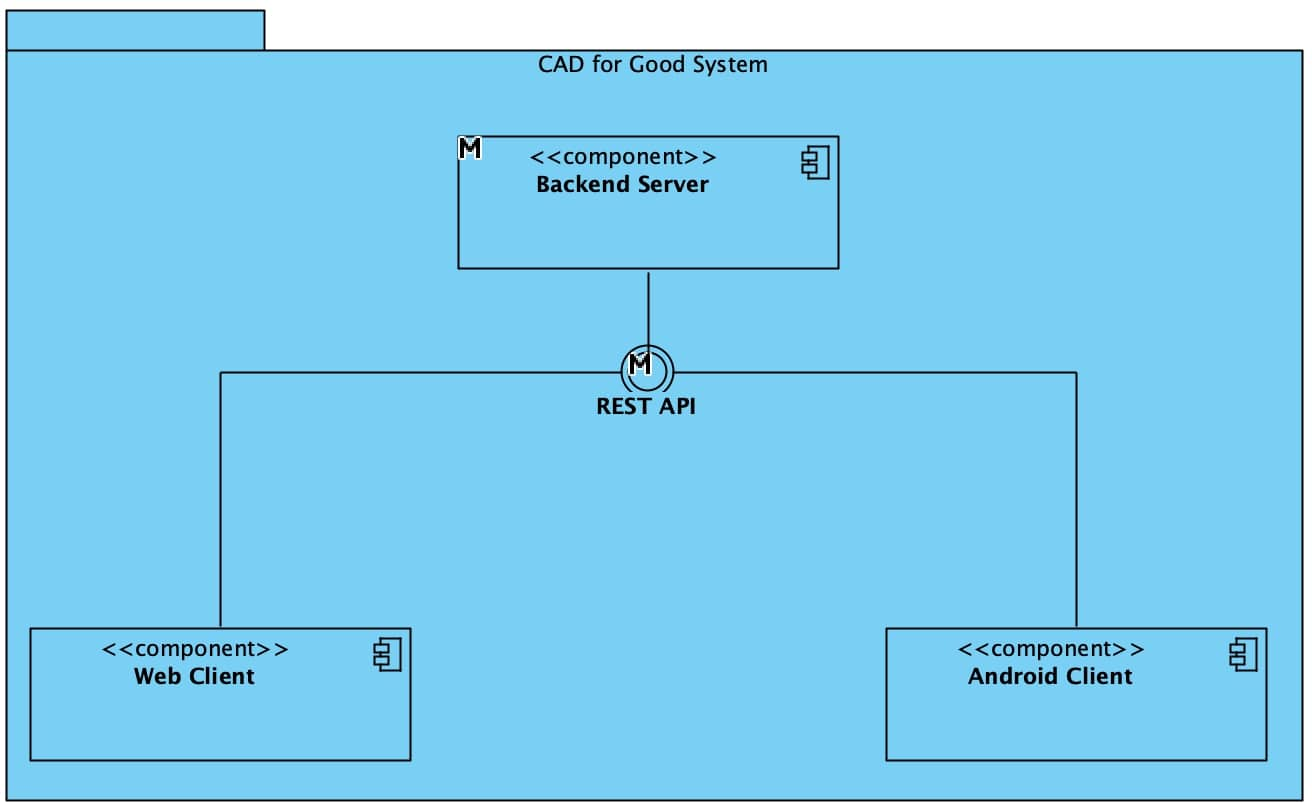
\includegraphics[width=1.0\linewidth]{pesti-report/images/global-system.jpg}
	\caption{System architecture}
	\label{fig:global-system}
\end{figure}
\\

The objective was to build clients with a focus on user-experience and which felt faster than directly requesting the EPCON servers.

\section{Implementation description}

To decide which technologies and frameworks we would use in order to develop the whole system we started by gathering information about the technical skills and previous experiences each of us had. We strongly thought about it and tried to not be influenced by the framework hype that exists nowadays. Many times during softwares development people put too much emphasis on the technology rather than the solution. We all agreed that we would go with the technologies that we felt comfortable with and not the ones that seemed better.
\\ \\
After this information gathering we decided to go with Node.js and Express for the backend API, JavaScript and React for the web client and Kotlin and Java for the Android client.

\\ \\
\begin{figure}[!h]
	\centering
	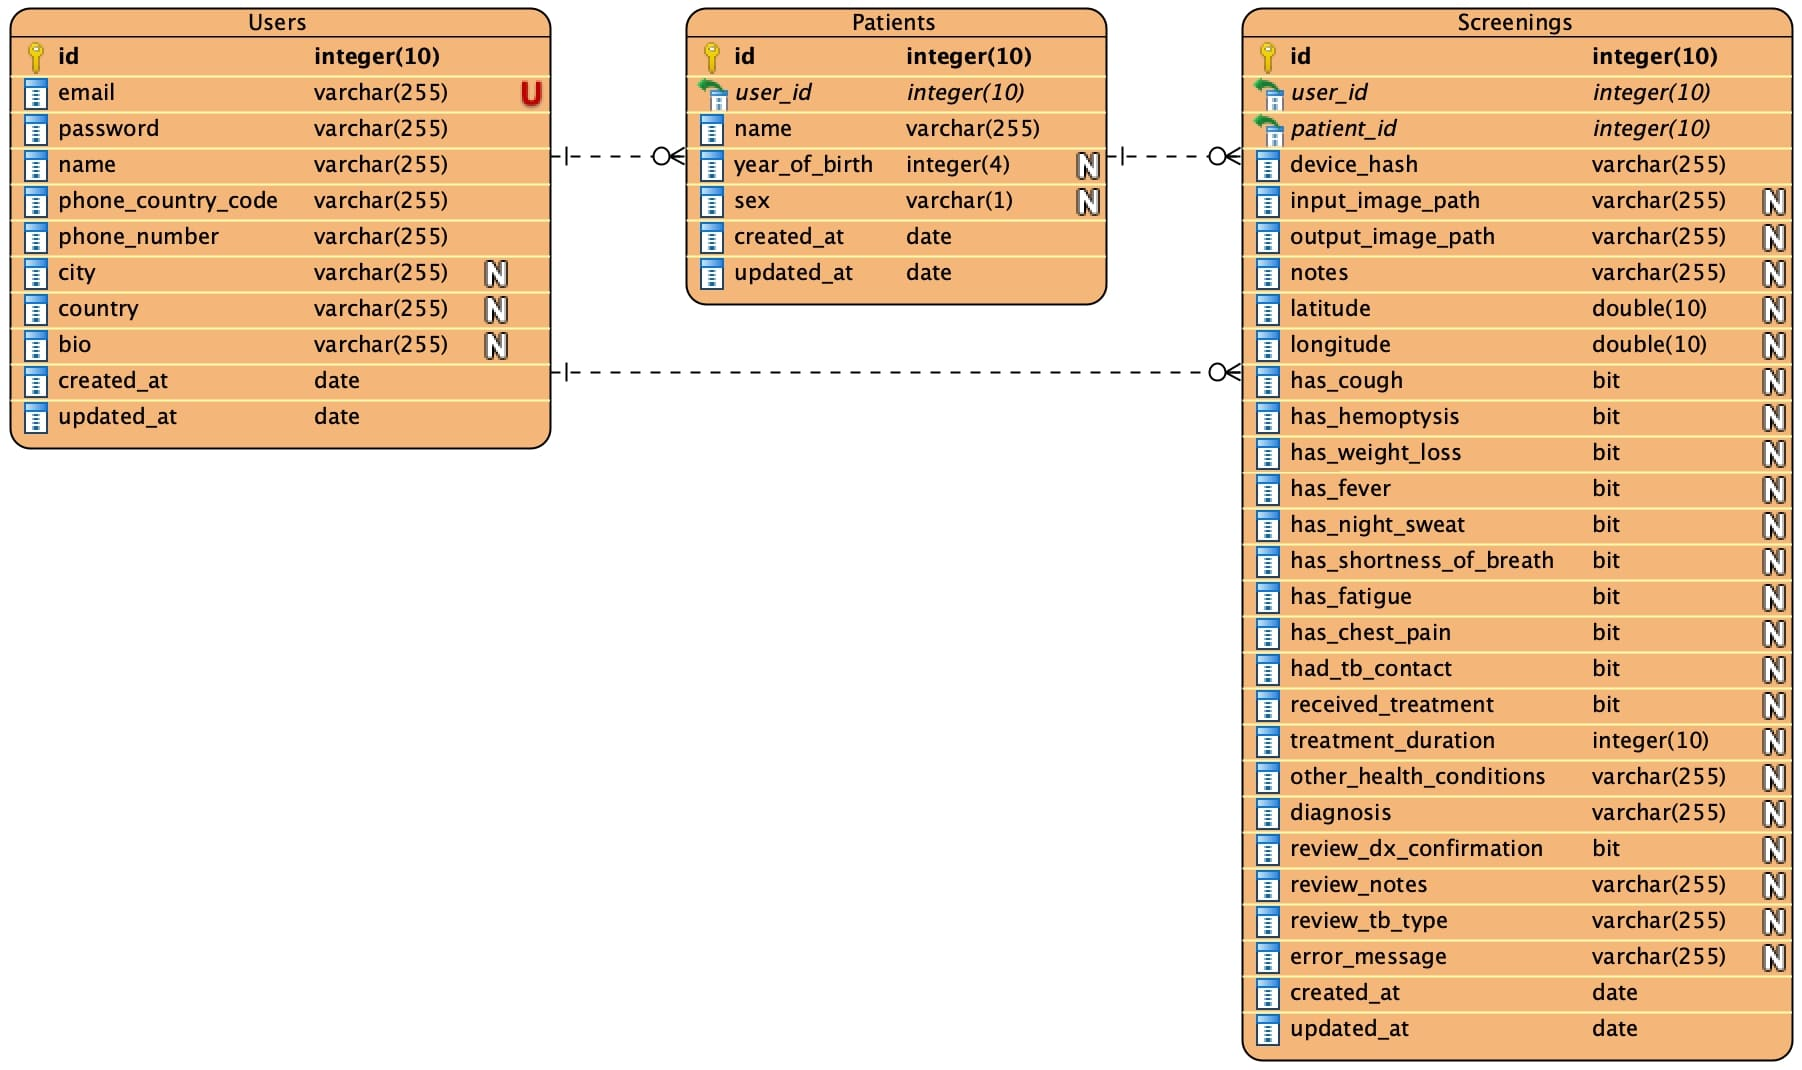
\includegraphics[width=1.0\linewidth]{pesti-report/images/database-schema.jpg}
	\caption{Database schema}
	\label{fig:database-schema}
\end{figure}
\\


\section{Backend architecture}


\\ \\
\begin{figure}[!h]
	\centering
	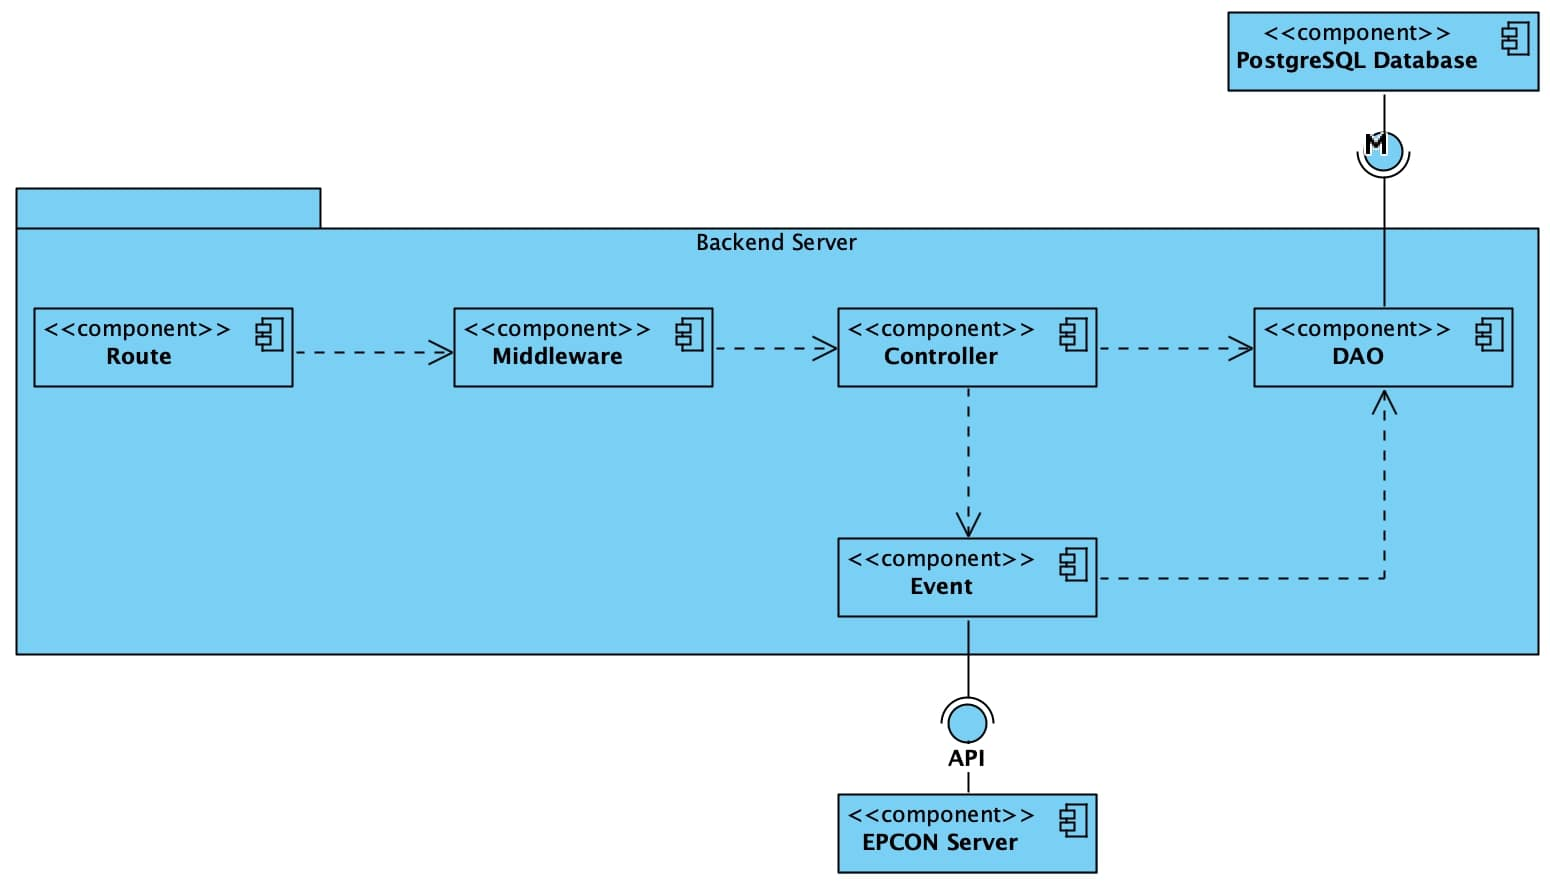
\includegraphics[width=1.0\linewidth]{pesti-report/images/backend-server-architecture.jpg}
	\caption{Backend server architecture}
	\label{fig:backend-server-architecture}
\end{figure}
\\


\section{Web client structure}

\\ \\
\begin{figure}[!h]
	\centering
	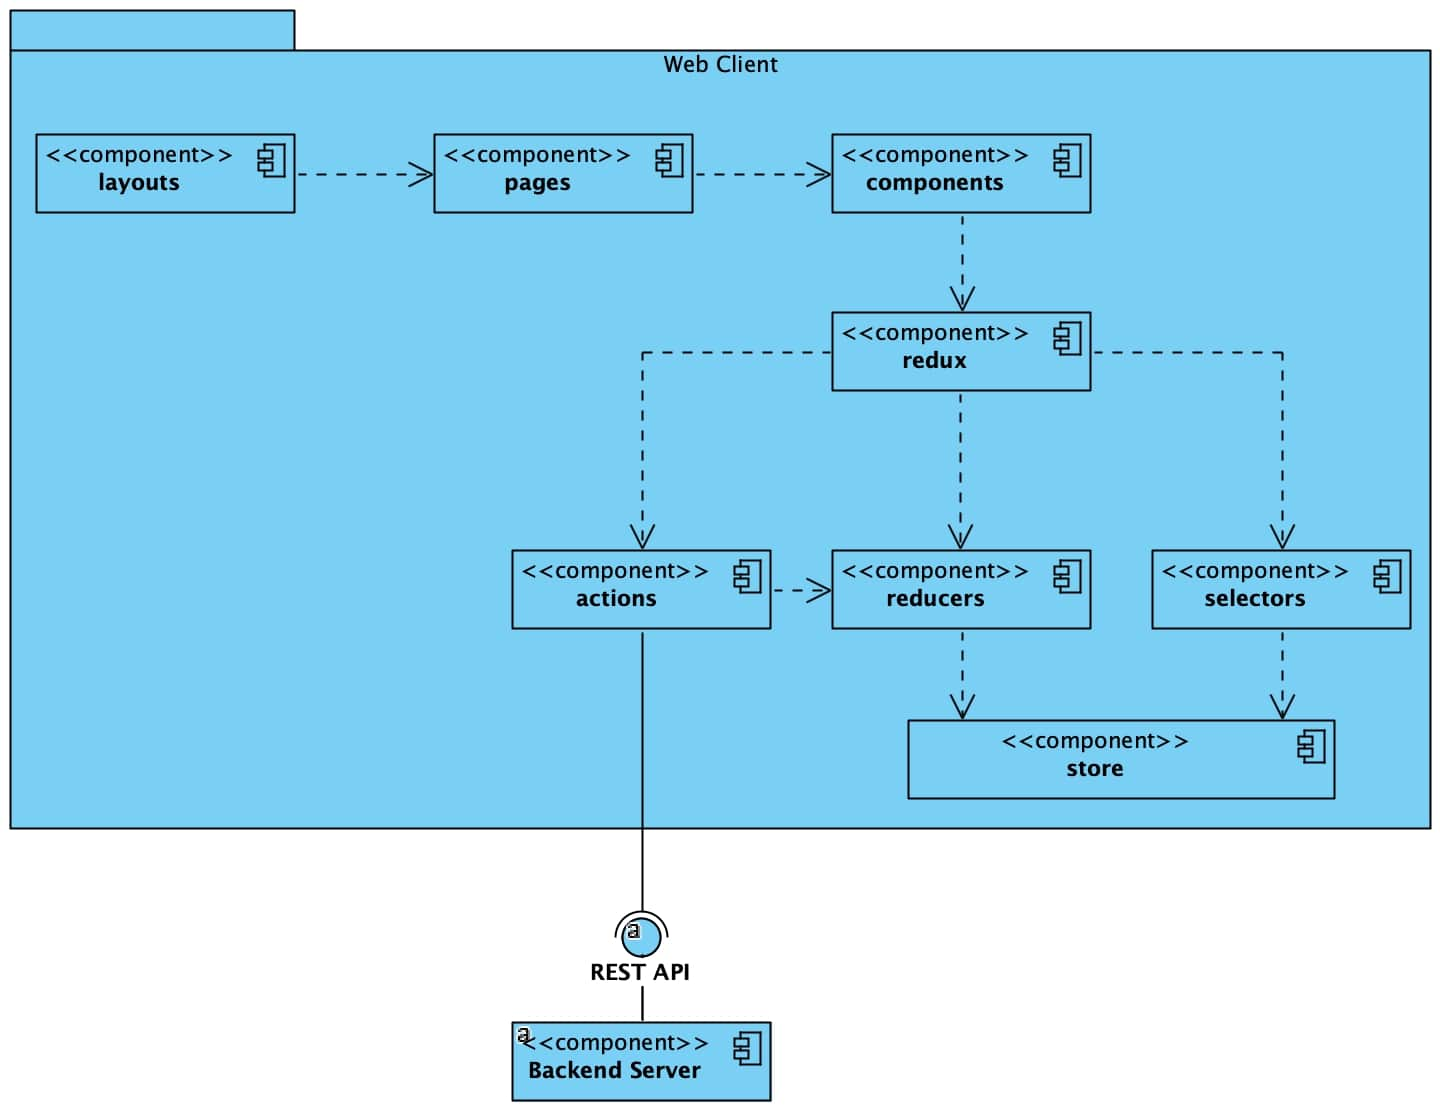
\includegraphics[width=1.0\linewidth]{pesti-report/images/web-client-structure.jpg}
	\caption{Web client structure}
	\label{fig:web-client-structure}
\end{figure}
\\


\section{Android client structure}


\\ \\
\begin{figure}[!h]
	\centering
	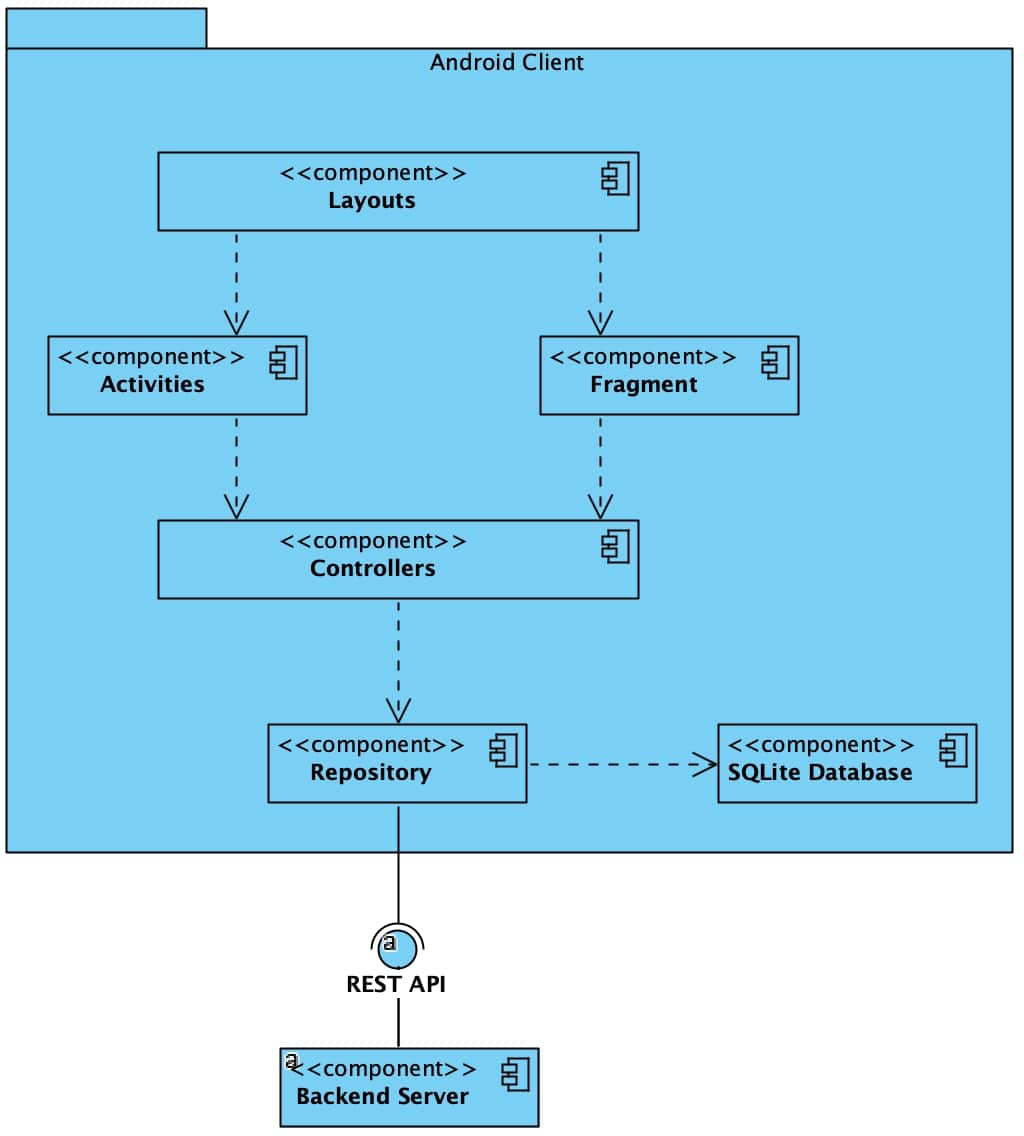
\includegraphics[width=1.0\linewidth]{pesti-report/images/android-client-structure.jpg}
	\caption{Android client structure}
	\label{fig:android-client-structure}
\end{figure}
\\




\section{Tests}


\\ \\
\begin{figure}[!h]
	\centering
	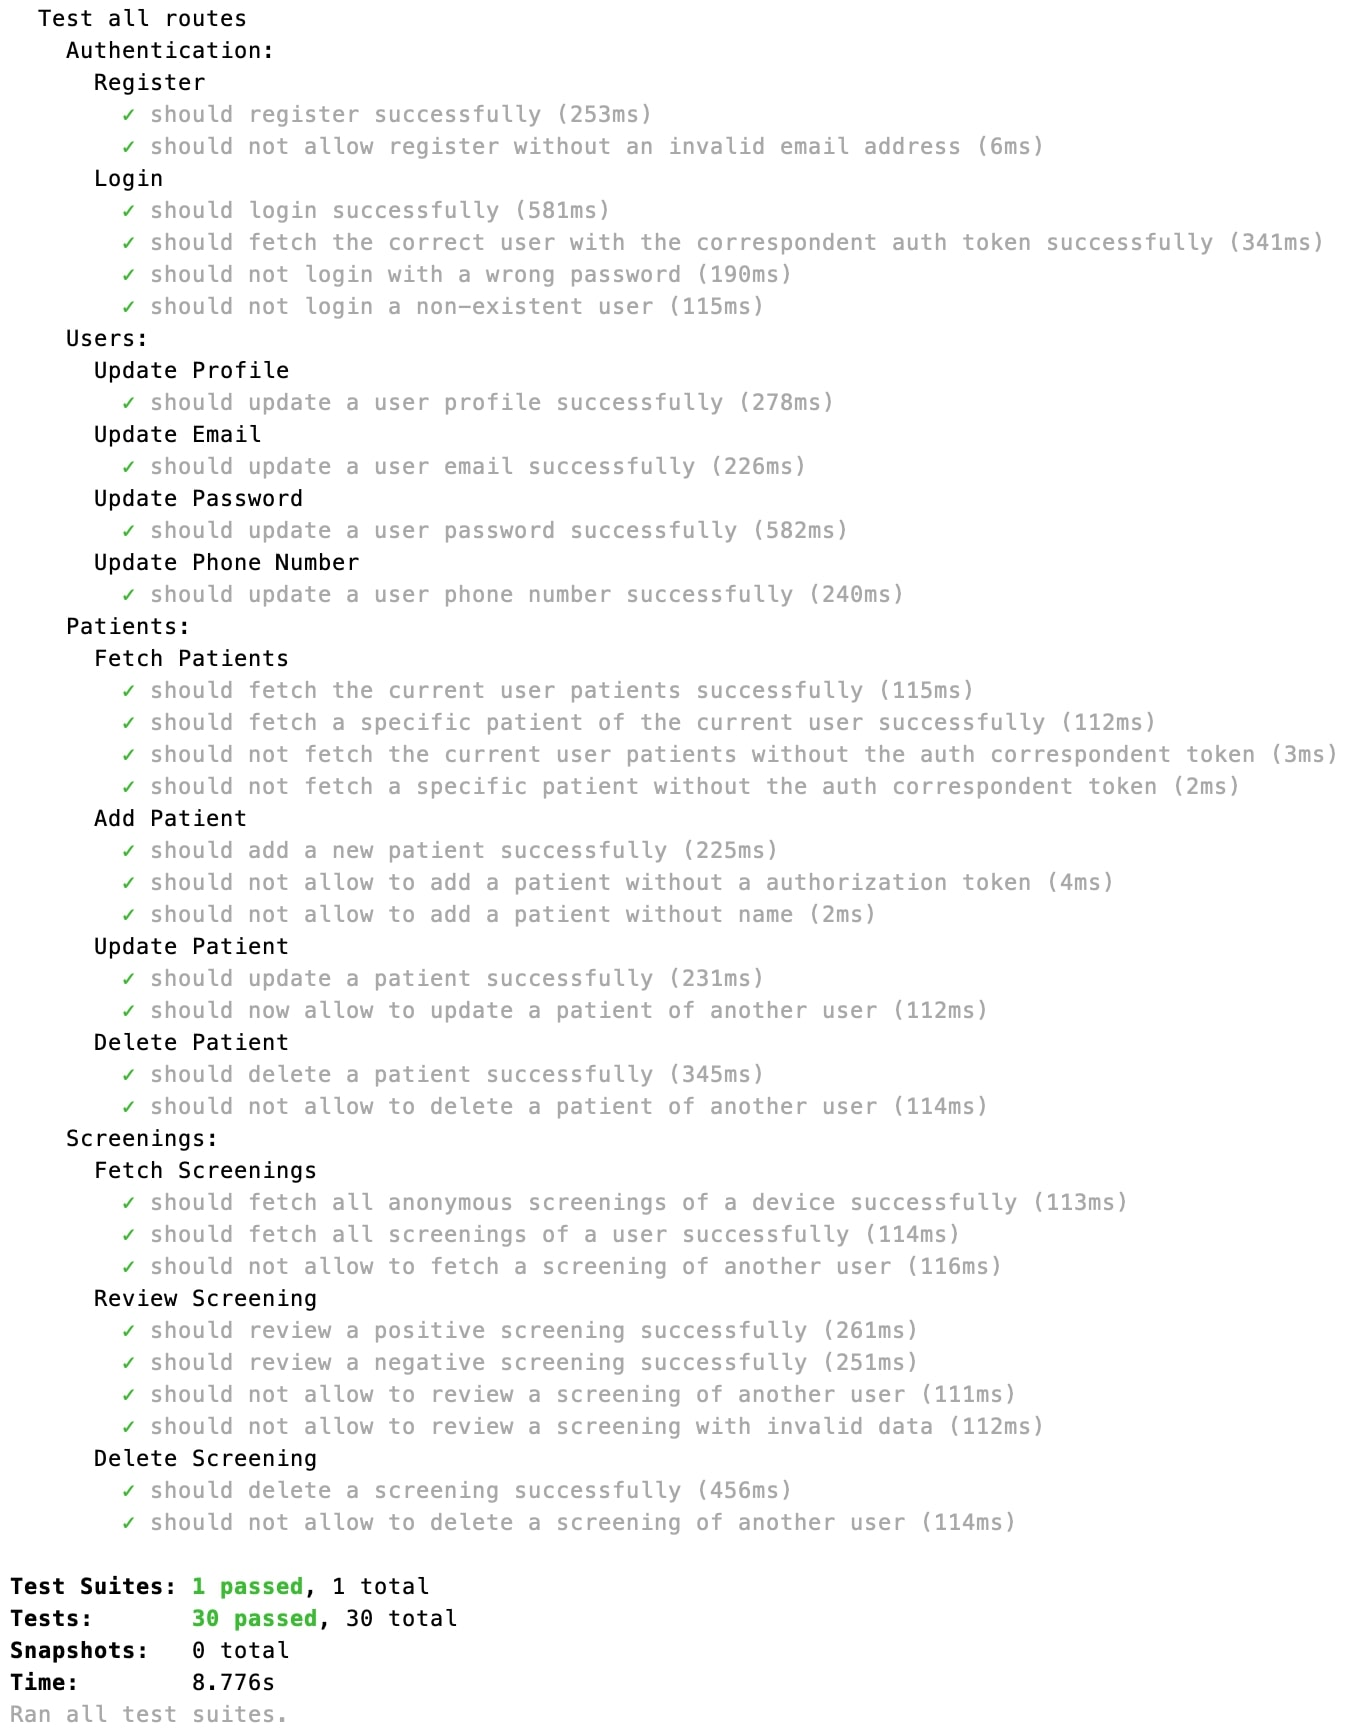
\includegraphics[width=1.0\linewidth]{pesti-report/images/unit-tests.jpg}
	\caption{Unit tests}
	\label{fig:unit-tests}
\end{figure}
\\

\section{Releases and deployment}

\section{Solution evaluation}

